\documentclass{beamer}

\usefonttheme{professionalfonts} % using non standard fonts for beamer
\usefonttheme{serif} % default family is serif

%\usepackage{hyperref}

%\usepackage{minted}

\usepackage{animate}

\usepackage{graphicx}

\def\Put(#1,#2)#3{\leavevmode\makebox(0,0){\put(#1,#2){#3}}}

\usepackage{color}

\usepackage{tikz}

\usepackage{amssymb}

\usepackage{enumerate}


\newcommand\blfootnote[1]{%

  \begingroup

  \renewcommand\thefootnote{}\footnote{#1}%

  \addtocounter{footnote}{-1}%

  \endgroup

}

\makeatletter

%%%%%%%%%%%%%%%%%%%%%%%%%%%%%% Textclass specific LaTeX commands.

 % this default might be overridden by plain title style

 \newcommand\makebeamertitle{\frame{\maketitle}}%

 % (ERT) argument for the TOC

 \AtBeginDocument{%

   \let\origtableofcontents=\tableofcontents

   \def\tableofcontents{\@ifnextchar[{\origtableofcontents}{\gobbletableofcontents}}

   \def\gobbletableofcontents#1{\origtableofcontents}

 }

%%%%%%%%%%%%%%%%%%%%%%%%%%%%%% User specified LaTeX commands.

\usetheme{Malmoe}

% or ...

\useoutertheme{infolines}

\addtobeamertemplate{headline}{}{\vskip2pt}



\setbeamercovered{transparent}

% or whatever (possibly just delete it)

\makeatother

\begin{document}
\title[DCEL report]{RIDIR Report}
\author[AC]{Andres Calderon}
\institute[Winter'20]{University of California, Riverside}
\makebeamertitle
\newif\iflattersubsect

\AtBeginSection[] {
    \begin{frame}<beamer>
    \frametitle{Outline} 
    \tableofcontents[currentsection]  
    \end{frame}
    \lattersubsectfalse
}

\AtBeginSubsection[] {
    \begin{frame}<beamer>
    \frametitle{Outline} 
    \tableofcontents[currentsubsection]  
    \end{frame}
}

\begin{frame}{CA subset [CGAL]...}
    \centering
	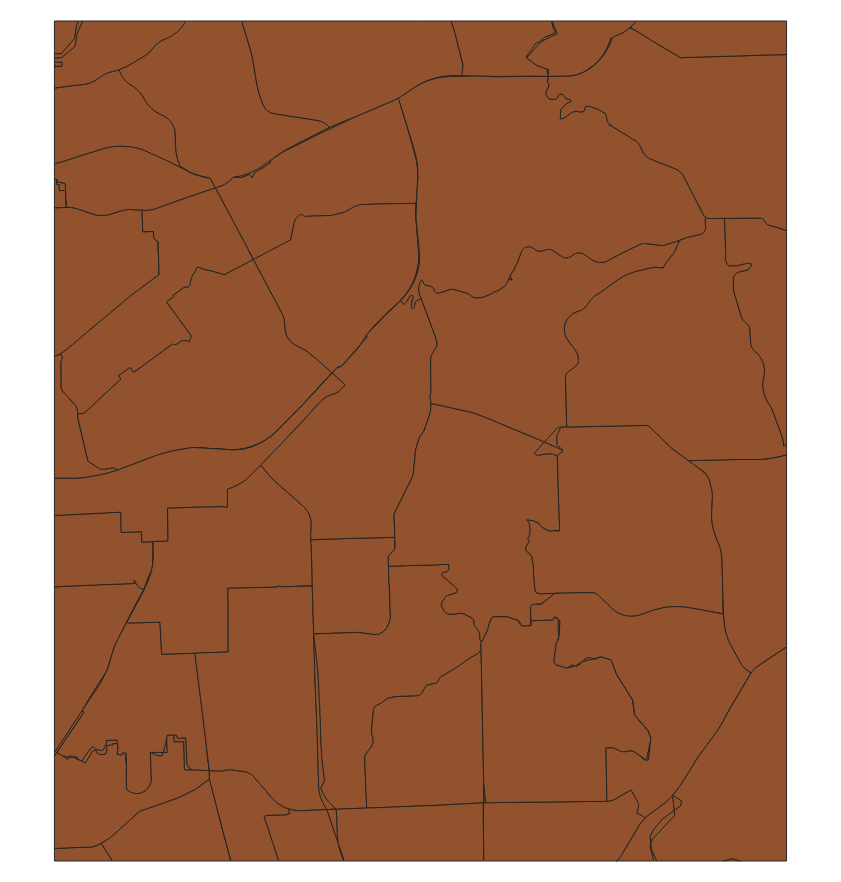
\includegraphics[width=0.625\textwidth]{figures/CA_Faces_CGAL}
\end{frame}
\begin{frame}{CA subset [RIDIR]...}
    \centering
	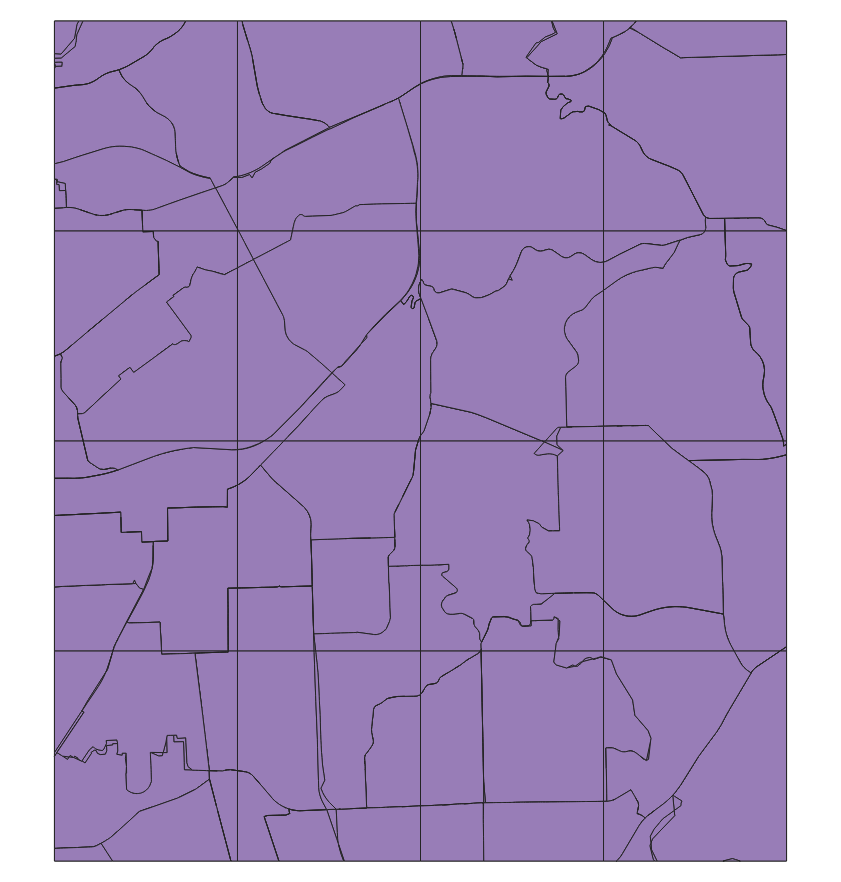
\includegraphics[width=0.625\textwidth]{figures/CA_Faces_RIDIR}
\end{frame}

\begin{frame}{Phili dataset [CGAL]...}
    \centering
	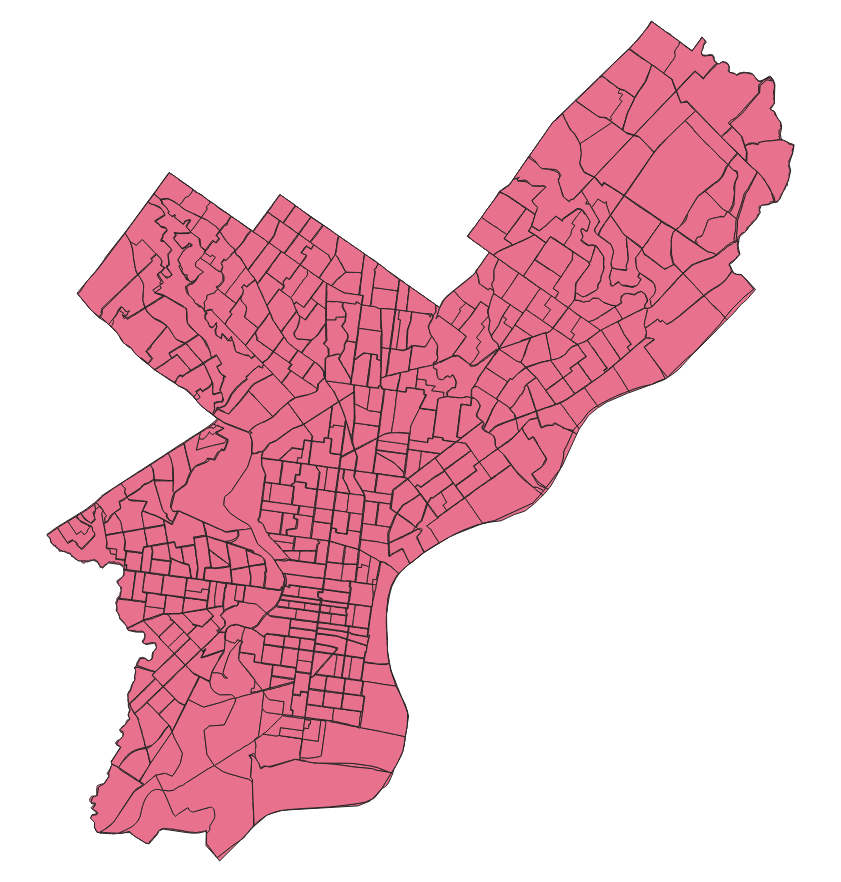
\includegraphics[width=0.625\textwidth]{figures/Phili_Faces_CGAL}
\end{frame}
\begin{frame}{Phili dataset [RIDIR]...}
    \centering
	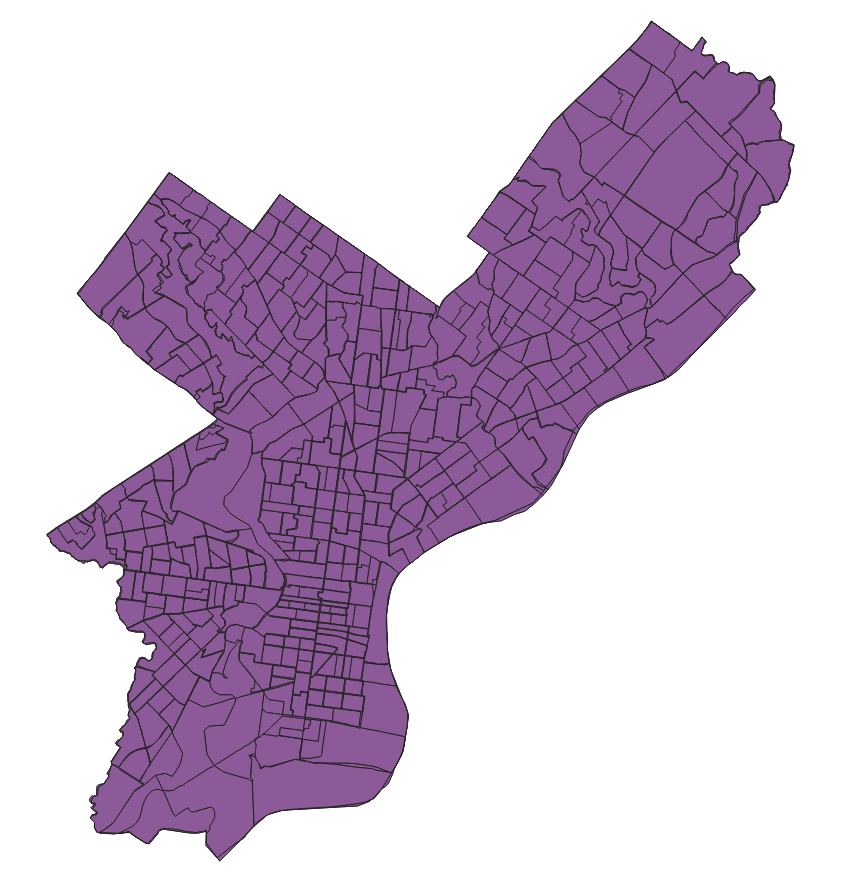
\includegraphics[width=0.625\textwidth]{figures/Phili_Faces_RIDIR}
\end{frame}
\begin{frame}{Phili dataset [CGAL] details...}
    \centering
	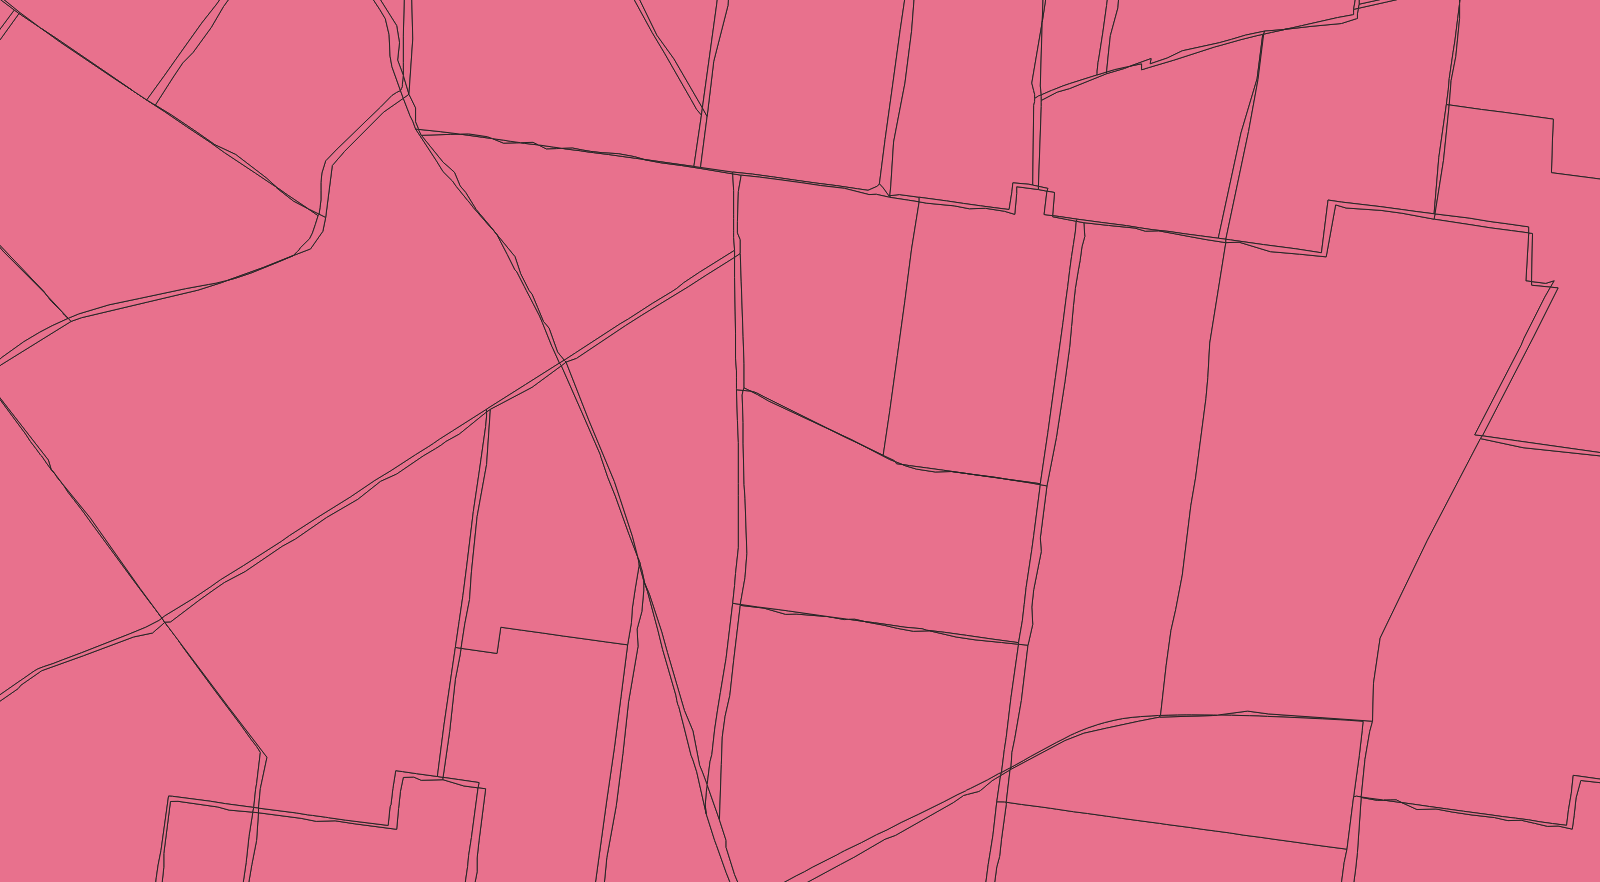
\includegraphics[width=0.9\textwidth]{figures/Phili_Faces_CGAL_details}
\end{frame}
\begin{frame}{Phili dataset [RIDIR] details...}
    \centering
	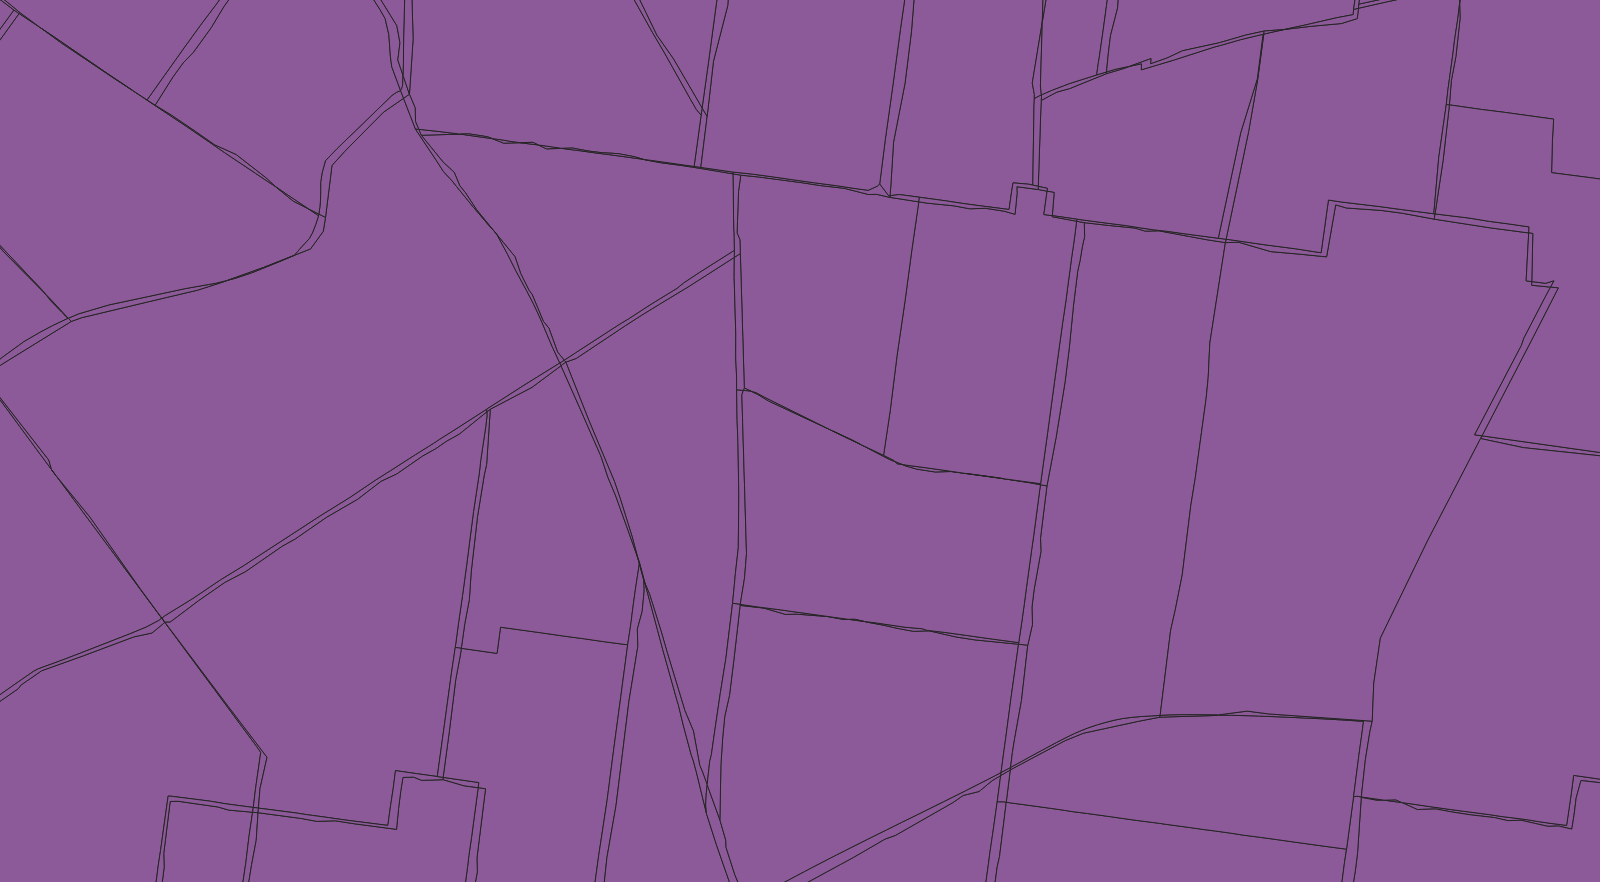
\includegraphics[width=0.9\textwidth]{figures/Phili_Faces_RIDIR_details}
\end{frame}

\begin{frame}{What's next?}
    \begin{itemize}
        \item I still have a bug at the moment of the merge in the full CA dataset.  Currently working on that...
        \item Tuning cluster parameters...
        \item Benchmarking with sequential tool...
    \end{itemize}
\end{frame}

\end{document}
